\chapter{Proceso}

\section{El Seguro}	
\setlength{\parskip}{5mm}
	El seguro constituye la forma más perfecta y técnicamente eficaz para la cobertura de riesgos -transformando los individuales en colectivos- y transfiriéndolos a una organización -el asegurador- estructurada con la técnica y operativa adecuadas para garantizar su compensación, en caso de ocurrir el evento.
\setlength{\parskip}{0mm}

\subsection{Contrato del seguro}
\setlength{\parskip}{5mm}

	El contrato de seguro, es aquel contrato mediante el cual una persona llamada asegurador se obliga, a cambio de una suma de dinero, conocida como prima, a indemnizar a otra llamada asegurado o a la persona que este designe, beneficiario, de un perjuicio o daño que pueda causar un suceso incierto. De tal manera que la suma objeto de indemnización, que fue pactada expresamente, sea pagada cuando ocurra el suceso o riesgo cubierto por el seguro. (\citeauthor{contratobib}, \citeyear{contratobib})

\setlength{\parskip}{0mm}

% \subsubsection{Características}

% \begin{itemize}

% 	\item Es un acto de comercio.- Efectivamente el contrato de seguro constituye un contrato mercantil, regulado en el Código de Comercio y en otros aspectos supletoriamente por la legislación civil.

% 	\item Es un contrato solemne.- El contrato de seguro es solemne, ya que su perfeccionamiento se produce a partir del momento en que el asegurador suscribe la póliza, la firma del asegurador sirve para solemnizar el acuerdo previo de voluntades entre las partes contratantes, respecto a los elementos del seguro.

% 	\item Es un contrato bilateral.- En razón de que genera derechos y obligaciones para cada uno de los sujetos contratantes, GARRIGUES al respecto señala : "..el tomador de seguros se obliga a pagar la prima y el asegurador se obliga a una prestación pecuniaria: si bien esta prestación esta subordinada a un evento incierto, cual es la realización del siniestro".

% 	\item Es un contrato oneroso.- Es oneroso, porque significa para las partes un enriquecimiento y empobrecimiento correlativos. "Por cuanto al tomador del seguro se le impone la obligación de pagar la prima y al asegurador la asunción del riesgo de la que deriva la prestación del pago de la indemnización de la que queda liberado si no se ha pagado la prima antes del siniestro".

% 	\item Es un contrato aleatorio.- Es aleatorio porque tanto el asegurado como el asegurador están sometidos a una contingencia que puede representar para uno una utilidad y para el otro una pérdida. Tal contingencia consiste en la posibilidad de que se produzca el siniestro. Al respecto el profesor MONTOYA dice : " El carácter aleatorio del contrato no desaparece por el hecho de que las compañías aseguradoras dispongan de tablas estadísticas que les permite determinar el costo de los riesgos, en función de lo cual fijan el importe de las primas…. osea que si bien la actividad aseguradora en si es cada vez menos riesgosa en la medida del perfeccionamiento de los medios para determinar la frecuencia de los riesgos, el contrato sigue siendo aleatorio tratándose de cada contrato aislado y respecto del asegurado".

% 	\item Es un contrato de ejecución continuada.- Por cuanto los derechos de las partes o los deberes asignados a ellas se van desarrollando en forma continua, a partir de la celebración del contrato hasta su finalización por cualquier causa.

% 	\item Es un contrato de adhesión.- El seguro no es un contrato de libre discusión sino de adhesión. Las cláusulas son establecidas por el asegurador, no pudiendo el asegurado discutir su contenido, tan sólo puede aceptar o rechazar el contrato impuesto por el asegurador. Sólo podrá escoger las cláusulas adicionales ofrecidas por el asegurador, pero de ninguna manera podrá variar el contenido del contrato. Pero todo esto dependerá de la voluntad y de la flexibilidad que tenga cada empresa aseguradora.

% \end{itemize}




\subsection{Funciones del Seguro}
\setlength{\parskip}{5mm}

Existen diferentes funciones del seguro, entre ellas tenemos: 

\setlength{\parskip}{0mm}

\subsubsection{Funciones sociológicas del seguro}

\begin{itemize}
	\item Fomenta la  protección de todos los miembros de una familia o individuos.

	\item Estimula el sentido de responsabilidad frente a terceros, esencial para: abrir nuevas empresas, realizar nuevas inversiones, crear empleo, etc.

	\item Contribuye a la estabilidad social protegiendo contingencias derivadas de la vejez y enfermedades o 
	accidentes.

	\item Financia la prevención de riesgos mediante la reducción de primas. Así, aparte de la colaboración del seguro con otros sectores, en el aspecto individual se destaca el espíritu de previsión representado en el interés que muestra en la prevención de las consecuencias desfavorables de un evento.

\end{itemize}

\subsubsection{Funciones económicas del seguro}

\begin{itemize}
	\item Contribuye positivamente al desarrollo económico al eliminar riesgos y estabilizar los resupuestos económicos. Por esto, debe desarrollarse paralelamente al resto de las actividades económicas.

	\item El seguro es la única actividad económica que posee capacidad para generar ahorro y financiación de inversiones a largo plazo.% Existen otras instituciones financieras que aportan ahorro a largo plazo pero sólo el seguro lo hace con un esquema de ahorro y financiando un tipo de inversión (global y sistemática) sustancialmente distintos a los utilizados habitualmente por otros intermediarios.

\end{itemize}

\subsubsection{Funciones laborales del seguro}

\begin{itemize}

	\item El seguro participa en la consecución de empleo directo e indirecto. Se estima que en España casi 49.000 familias “viven del seguro” (empleados, agentes, corredores, peritos, liquidadores, abogados, actuarios y otros profesionales) y que el sector está financiando alrededor de 600.000 puestos de trabajo estable.

\end{itemize}

\subsection{Póliza de seguro}
\setlength{\parskip}{5mm}

	La póliza es el documento principal del contrato de seguro, en donde constan los derechos y obligaciones de las partes, es un documento privado redactado en varios folios. Las condiciones generales están impresas, mientras las condiciones particulares están normalmente mecanografiadas. 

	% http://www.monografias.com/trabajos17/contrato-seguro/contrato-seguro.shtml#poliza#ixzz4M9kcfgxe

\setlength{\parskip}{0mm}


\subsection{Seguro de Vehículo}
\setlength{\parskip}{5mm}

Este tipo de seguro puede amparar tanto los daños propios como los daños causados a un tercero.

\begin{itemize}
	\item Cobertura Amplia: La aseguradora se compromete a  indemnizar al Asegurado, en exceso del deducible y hasta la suma asegurada indicada en el Cuadro Póliza, los daños materiales que sufra el Vehículo Asegurado en el período de vigencia de la Póliza, mientras el vehículo se encuentre en circulación, reposo o en transporte dentro de la República Bolivariana de Venezuela, que ocasione un Daño Parcial, General o No Recuperable, salvo aquellos casos expresamente excluidos en esta Póliza.

	\item Cobertura de indemnización por robo del vehículo:La aseguradora se compromete a indemnizar al Asegurado, en caso de quedar privado del uso del Vehículo Asegurado, como consecuencia directa de Robo o hurto, una cantidad diaria, desde el día en que se hayan cumplido los requisitos establecidos para notificar el reclamo, de acuerdo con lo establecido en las Condiciones Particulares de la póliza, hasta el día en que:

	a) La Empresa de Seguros haga efectiva la indemnización correspondiente, una vez transcurrido el plazo previsto en las Condiciones Generales de esta Póliza.

	b) Se haya recuperado el Vehículo Asegurado en caso robo o hurto. De ser el Asegurado quién recupere el Vehículo Asegurado, se compromete a comunicarlo por escrito a la Empresa de Seguros.

	Si el Vehículo Asegurado recuperado requiere reparación por daños sufridos a causa del robo o del hurto, la aseguradora continuará indemnizando la cantidad diaria hasta la fecha prevista para la entrega del mismo. En ningún caso, la indemnización superará el monto de los días o suma asegurada para esta cobertura indicado en el cuadro-recibo de la póliza.


	\item Cobertura de responsabilidad civil ( Daños a terceros): La Aseguradora se compromete a indemnizar la responsabilidad que pudiera corresponder al propietario o conductor del vehículo asegurado, por lesiones o daños a terceros dentro de Venezuela de acuerdo a la ley y reglamento de tránsito vigente hasta los límites indicados en el cuadro de la póliza.

	\item Asistencia legal y/o defensa penal: Al ocurrir un accidente de transito, esta póliza cubre los gastos por asistencia legal para liberar al conductor y vehículo en caso de ser detenidos, así como todos los gastos correspondientes a su defensa penal si es necesario. Está también cubre los casos de demanda en contra del asegurado.


	\item Cobertura de accidentes personales para ocupantes de vehículos: La Aseguradora se compromete a indemnizar al Asegurado o Beneficiario,  la suma asegurada indicada en el Cuadro Póliza, por las lesiones corporales que afecten la integridad física de los Ocupantes del Vehículo Asegurado, a consecuencia de un accidente amparado por la Póliza mientras se encuentren dentro, subiendo o bajando del Vehículo Asegurado y bajo las Condiciones estipuladas en las condiciones de la Póliza.


\end{itemize}

\setlength{\parskip}{0mm}

\subsection{El Perito}
\setlength{\parskip}{5mm}
	El Perito es esencial en el engranaje de la compañía de seguros, pero para conocer la verdadera dimensión del trabajo del perito, analizamos sus funciones, que se resumen en tres grandes apartados:


\subsubsection{Aspectos técnicos}
\begin{itemize}

\item Valoración económica de los daños, elaborando la peritación y realizando la propuesta de indemnización a la compañía de seguros. Determinación del valor del bien asegurado, como, por ejemplo, el
valor venal, el valor de mercado, el valor de los restos y la propuesta del importe líquido de la indemnización, cuando se ha producido un siniestro total o una pérdida total.

\item Verificación de siniestros, para la realización de informes de uso interno para la compañía de seguros con la justificación técnica de la ocurrencia del siniestro. Pueden ser informes de rehúses parciales o totales, que pueden aportarse como prueba en un juicio. Los informes de reconstrucción de accidentes de tráfico, a partir de huellas y vestigios, mediante cálculos físicos y matemáticos, pueden ser también un apoyo para la determinación de la culpabilidad en el juicio. 

\item Revisión de riesgos, para la contratación de nuevas pólizas de vehículos de segunda mano con coberturas de daños propios, lunas, etc.

\item Control de calidad de la reparación, mediante la comprobación, en primer lugar, de que la reparación se ha llevado conforme a la peritación en todas y cada una de las partidas asignadas por el perito; a continuación, que la reparación se ha realizado con las debidas garantías técnicas, de calidad y seguridad para los ocupantes del vehículo. Por último, se analizarán los defectos en la reparación, para que sean subsanados por el taller.

\item Averías mecánicas: valoración y peritación de los daños mecánicos bajo la cobertura de pólizas de vehículos de renting y de pólizas de garantía de venta de vehículos usados.

\end{itemize}


\subsubsection{Aspectos administrativo-legales}
\begin{itemize}

\item Implicación en la tramitación del siniestro. El perito, en contacto con el tramitador y a través del sistema de gestión de la compañía de seguros, está al día de la tramitación de los siniestros, del tipo de pólizas que comercializa la compañía de seguros, de sus coberturas y exclusiones, de los convenios entre compañías y del conocimiento de la legislación de seguros.

\end{itemize}

\subsubsection{Aspecto negociador}
\begin{itemize}

\item El perito es la imagen de la compañía de seguros, ya que está en contacto con los asegurados, perjudicados, talleres, otras compañías, con lo que su actuación está sujeta a examen continuo, y su comportamiento, a ojos del asegurado, es, por extensión, el de la compañía de seguros. 

\item El perito debe aportar, en todo momento, argumentos y criterios técnicos en la negociación con el taller.

\item Ha de consensuar la peritación: debe llegar a acuerdos con el taller sobre todas y cada una de las partidas que componen una peritación.

\item Realiza asesoría legal: al estar en contacto con los asegurados y el taller, en muchas ocasiones, el perito se convierte en el asesor sobre los aspectos legales de los siniestros

\end{itemize}


(\citet{peritobib}, 2012)
\subsubsection{Inspección para asegurar un Vehículo}

En el proceso de peritaje y/o inspección es muy importante realizar un registro fotográfico del vehículo antes de comenzar a realizar las operaciones de diagnóstico.

Esto se realiza primero, porque es necesario el registro para el informe generado a las aseguradoras y/o el cliente y segundo, para evitar futuras reclamaciones a la hora determinar el proceso de inspección.

También se debe señalar la importancia que cumple la inspección al interior del vehículo, como soporte o elemento de consulta durante la atención de un siniestro para comparar características del vehículo y elementos de contenido.

En resumen el perito esta encargado de realizar diferentes tipos de inspecciones, para la inscripción de un vehículo nuevo en la aseguradora, tales como:

\begin{itemize}

	\item Registro Fotográfico.

	\item Inspección Mecánica.

	\item Inspección Latonería.

	\item Inspección Pintura.

	\item Inspección Vidrios.

	\item Inspección Chasis.

	\item Inspección Interiores y guarnecidos.

\end{itemize}

(\citet{peritoIVbib}, 2012)

\subsubsection{Caso de Estudio}

\begin{figure}[H]
\begin{center}
	\includegraphics[width=\textwidth,height=15cm]{img/proceso_sin_sistema.png}
\end{center}
\caption{Proceso Actual. (2016)}
\label{fig:proc_sin_sistema}
\end{figure}
\setlength{\parskip}{0mm}


\newpage

\subsubsection{Planilla de Suscripción}

\begin{figure}[H]
\begin{center}
	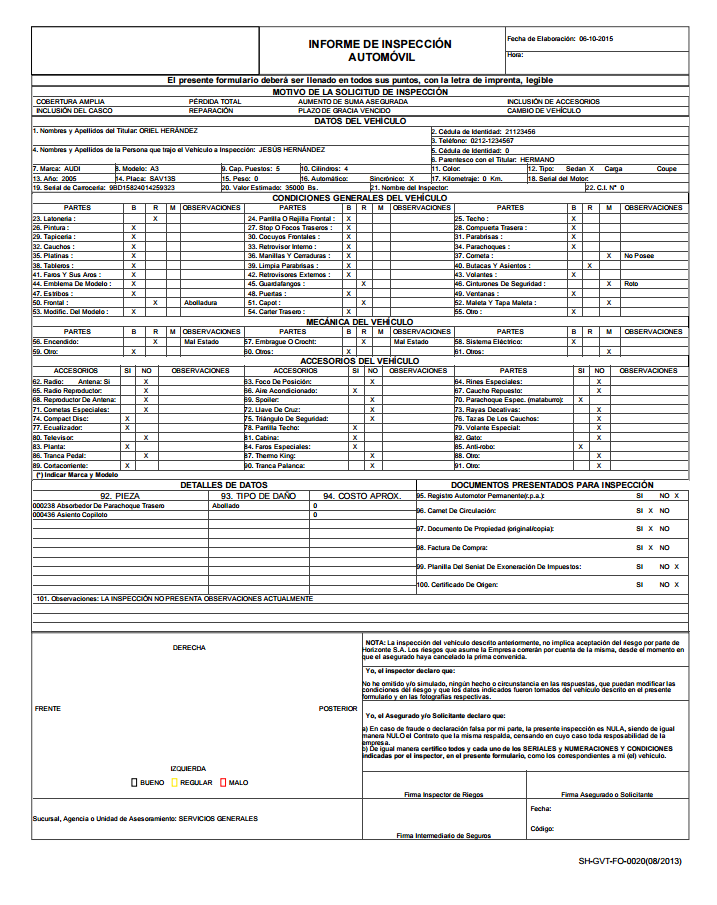
\includegraphics[width=\textwidth,height=18cm]{img/planilla_suscripcion.png}
\end{center}
\caption{Proceso de Suscripción. (2016)}
\label{fig:planilla_suscripcion}
\end{figure}
\setlength{\parskip}{0mm}